\documentclass[conference]{IEEEtran}
\IEEEoverridecommandlockouts
% The preceding line is only needed to identify funding in the first footnote. If that is unneeded, please comment it out.
\usepackage{cite}
\usepackage{amsmath,amssymb,amsfonts}
\usepackage{algorithmic}
\usepackage{graphicx}
\usepackage{textcomp}
\usepackage{xcolor}
\def\BibTeX{{\rm B\kern-.05em{\sc i\kern-.025em b}\kern-.08em
    T\kern-.1667em\lower.7ex\hbox{E}\kern-.125emX}}
\begin{document}
\title{Machine Learning\\
{\footnotesize \textsuperscript{*}Analyzing problems, designing a machine learning solution, implementing ML algorithms, and evaluating  data sets }
}

\author{\IEEEauthorblockN{1\textsuperscript{st} Saksham Saxena}
\IEEEauthorblockA{\textit{dept. name of organization (of Aff.)} \\
\textit{name of organization (of Aff.)}\\
City, Country \\
email address}
\and
\IEEEauthorblockN{2\textsuperscript{nd} Rushabh Doshi}
\IEEEauthorblockA{\textit{dept. name of organization (of Aff.)} \\
\textit{name of organization (of Aff.)}\\
City, Country \\
email address}
\and
\IEEEauthorblockN{3\textsuperscript{rd} Luke Beaulieu}
\IEEEauthorblockA{\textit{dept. name of organization (of Aff.)} \\
\textit{name of organization (of Aff.)}\\
City, Country \\
email address}
\and
\IEEEauthorblockN{4\textsuperscript{th} Utkarsh Patel}
\IEEEauthorblockA{\textit{dept. name of organization (of Aff.)} \\
\textit{name of organization (of Aff.)}\\
City, Country \\
email address}
}

\maketitle


\begin{abstract}
This paper presents the analysis and evaluation on data sets using machine learning techniques. Our method in this assignment consist of working with three data sets and implement ML algorithms on them to understand more about the field of machine learning and its applications in the real world. The three three data sets worked on in this project was  Boston housing, breast cancer, and Forest Covertype.
\end{abstract}

\begin{IEEEkeywords}
introduction, methodology, result, discussion, conclusion
\end{IEEEkeywords}

\section{Introduction}
The goal of this final project is to show that we have learned something in the class. It is an opportunity for us to explore ideas that we have see in the lectures and assignments and extend them. This project is a first steps towards research in machine learning or its applications. We will analyze problems, design a machine learning solution, implement ML algorithms, and evaluate them on three data sets (one for classification and one for regression from “Small Data Sets” and one data set – either classification or regression – from “Large Data Sets”).

\section{Problem and Data sets}
\subsection{Breast Cancer, logistic regression}\label{AA}
Breast cancer data set is a classification data set. The output variable of the cancer data was either malignant or benign .
%○ What are the important ideas/methods you explored?
%○ What ideas from the class did you use?
%○ Reporting the results (cross-validation, easy-to-read figures, etc)
%○ Do the results make sense?
%○ If you had much more time, how would you continue the project?

\begin{figure}[htbp]
\centerline{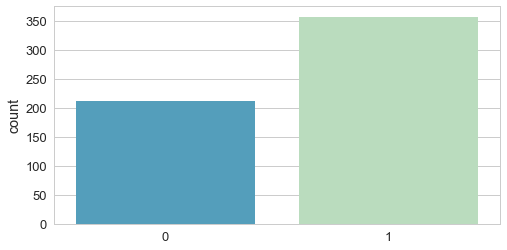
\includegraphics[width=50mm,scale=0.5]{imgs/output_16_1.png}}
\caption{0: Malignant 1: Benign}
\label{fig}
\end{figure}

Since this is a classification data set, it was important to go back and look at which methods I could and could not use to work with this data set. I chose logistic regression model in this case. The idea of logistic regression is that there is an optimal decision boundary that separates the two classes of cancer. From class, we learned methods to obtain that optimal decision boundary using cost function.

For the given training data, we want to find parameters $\Theta$ that are most likely by maximizing L($\Theta$). This is the maximum likelihood estimator.
\begin{figure}[htbp]
\centerline{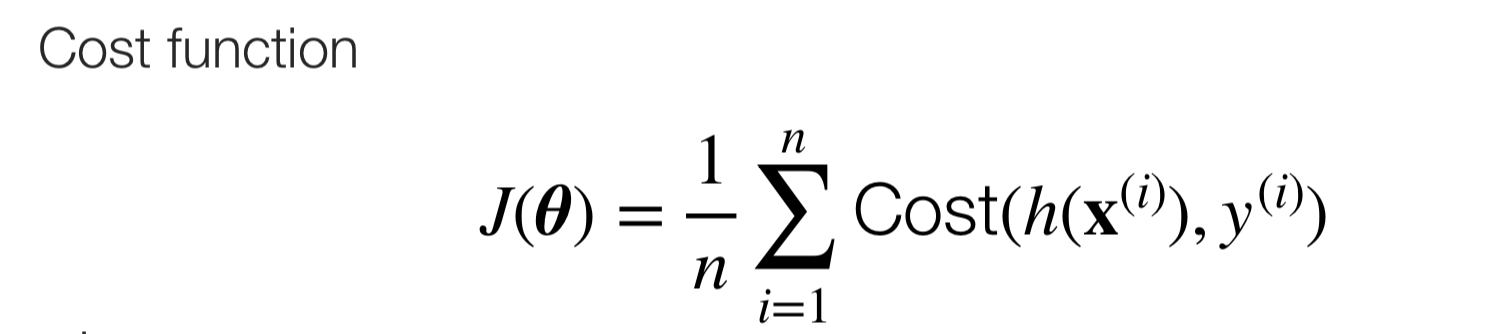
\includegraphics[width=50mm,scale=0.5]{imgs/cost_func}}
\label{fig}
\end{figure}

\begin{figure}[htbp]
\centerline{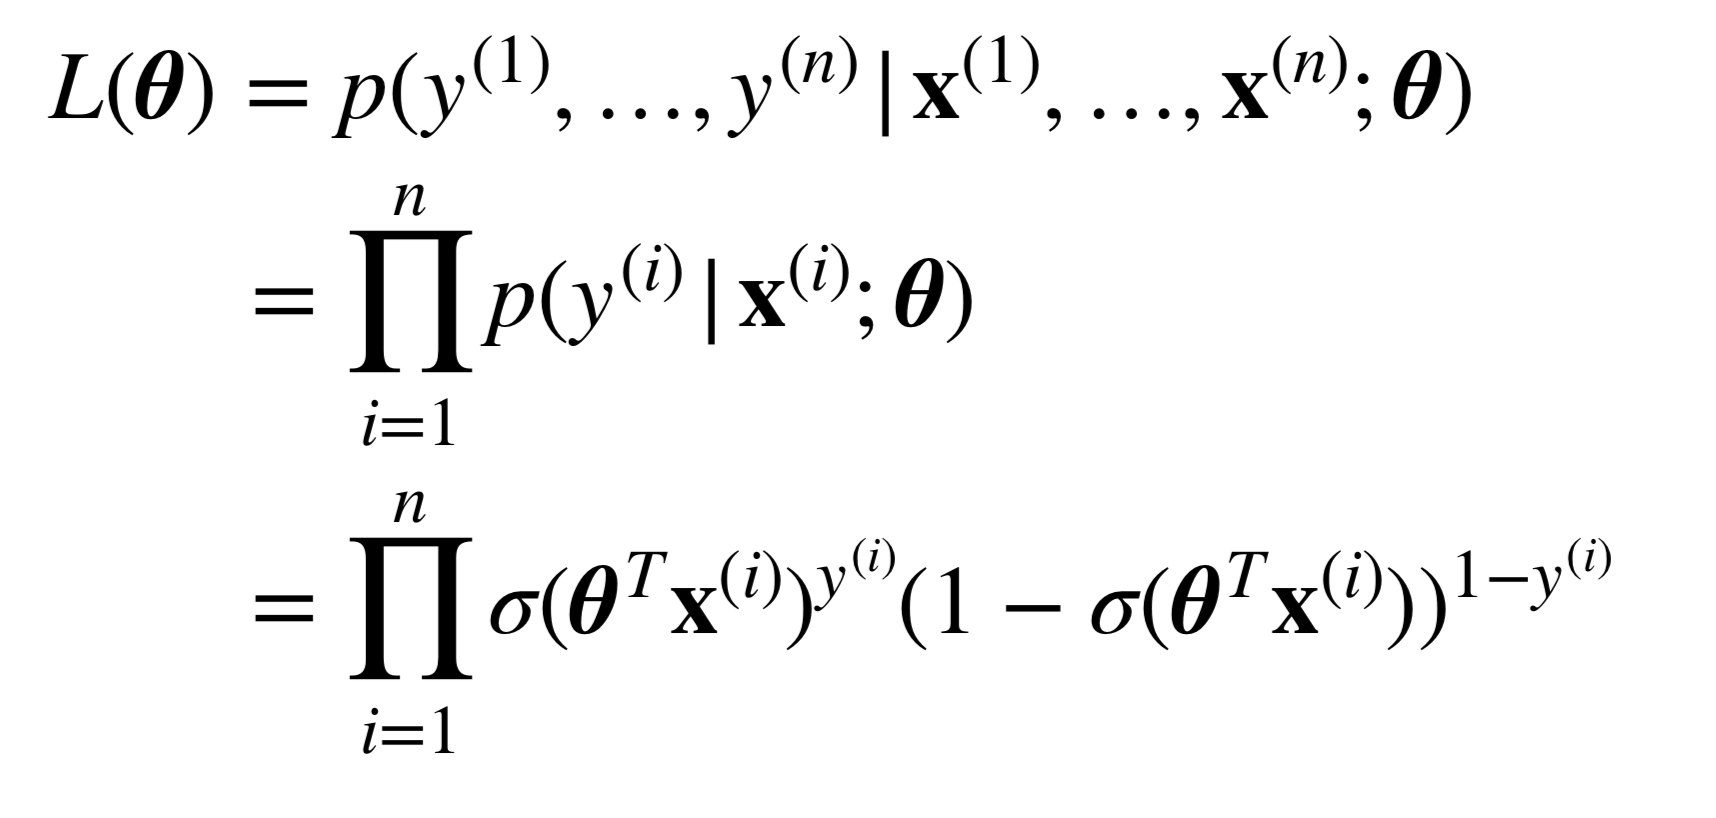
\includegraphics[width=50mm,scale=0.5]{imgs/max_like}}
\caption{maximum likelihood estimator function}
\label{fig}
\end{figure}
Knowing the likelihood function (above) for this given problem, we look for such $\Theta$ that maximizes the probability of obtaining the data we have. To find the $\Theta$, we have an optimization algorithm to find that $\Theta$.
\begin{figure}[htbp]
\centerline{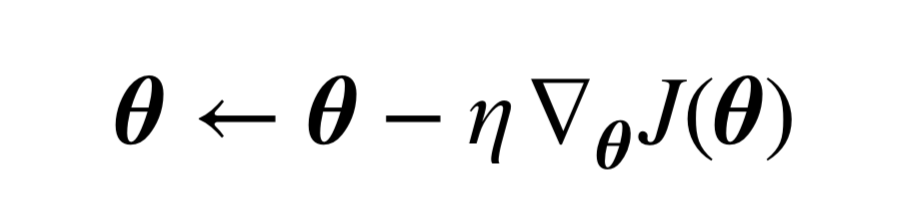
\includegraphics[width=50mm,scale=0.5]{imgs/gradient}}
\caption{gradient descend where n is the learning rate }
\label{fig}
\end{figure}
\newpage
Going through different learning rates and iterations, this leaves us with an optimal line that separates the two classification of breast cancer. *n is the learning rate and it determines how big of a step we get to the minimum point in the gradient descend.  
\noindent-Too big of a learning rate causes drastic updates which leads to divergent behavior. 
\noindent-Too small of a learning rate and it may take a lot of iterations to get to the minimum point. 
\begin{figure}[htbp]
\centerline{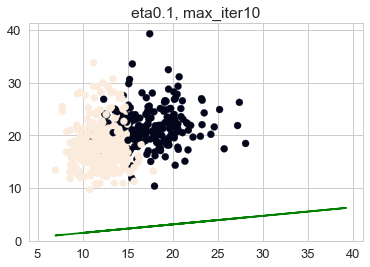
\includegraphics[width=50mm,scale=0.5]{imgs/output_20_1.png}}
\caption{Small learning rate and iteration}
\label{fig}
\end{figure}
\begin{figure}[htbp]
\centerline{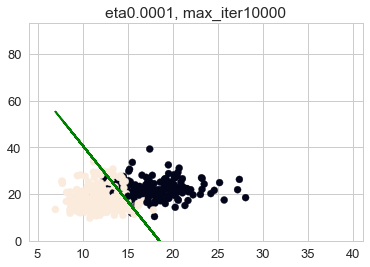
\includegraphics[width=50mm,scale=0.5]{imgs/output_20_16.png}}
\caption{Good learning rate and iteration}
\label{fig}
\end{figure}

Although I did not have enough time to find the numerical of the errors and accuracy, that is what I would have liked to do if i had more time.(doable using train  and test using a 40:60 split model)

The logistic model optimally draws the line between two classes of data, so these results (graphs) do make sense.

\subsection{Breast Cancer, Support Vector Machine}
%○ What are the important ideas/methods you explored?
%○ What ideas from the class did you use?
%○ Reporting the results (cross-validation, easy-to-read figures, etc)
%○ Do the results make sense?
%○ If you had much more time, how would you continue the project?
Support Vector Machine or SVM is another method for classification problems such at breast cancer. This works efficiently on datasets that are linearly separable, and so what SVM attempts to do is separate the data by a 'separating hyperplane'.  An SVM model is a representation of the examples as points in space, mapped so that the examples of the separate categories are divided by a clear gap that is as wide as possible. New examples are then mapped into that same space and predicted to belong to a category based on which side of the gap they fall. [wiki].

The methodology for SVM was to setup the data frame and use a train test 40:60 split. Then using the support vector classifier, or SVC model, I went to predict the accuracy of the model, how well it maps new data or examples for this data. 

\newpage
\begin{figure}[htbp]
\centerline{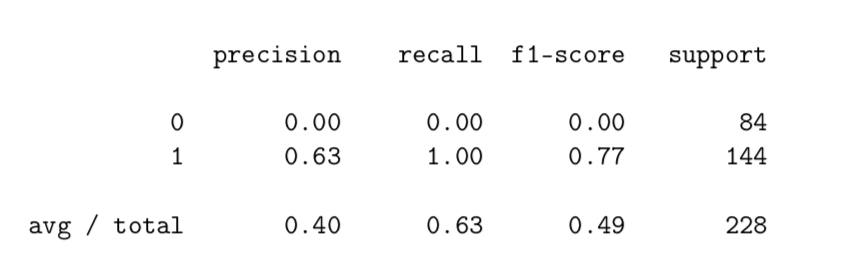
\includegraphics[width=50mm,scale=0.5]{imgs/class1}}
\caption{Prediction with no adjustment}
\label{fig}
\end{figure}
Obviously this was not a good prediction without training, adjustment, and normalizing the data. The model is fairly inaccurate. 

For the parameters of the SVC model, we want to use \textbf{grid search} to find the best parameter, specifically C and $\Gamma$. Grid search runs the same loop with cross-validations to find the best parameters. Once it has found the best combinations, it runs fit on all the data passed to build a single model using the best parameter setting.

\begin{figure}[htbp]
\centerline{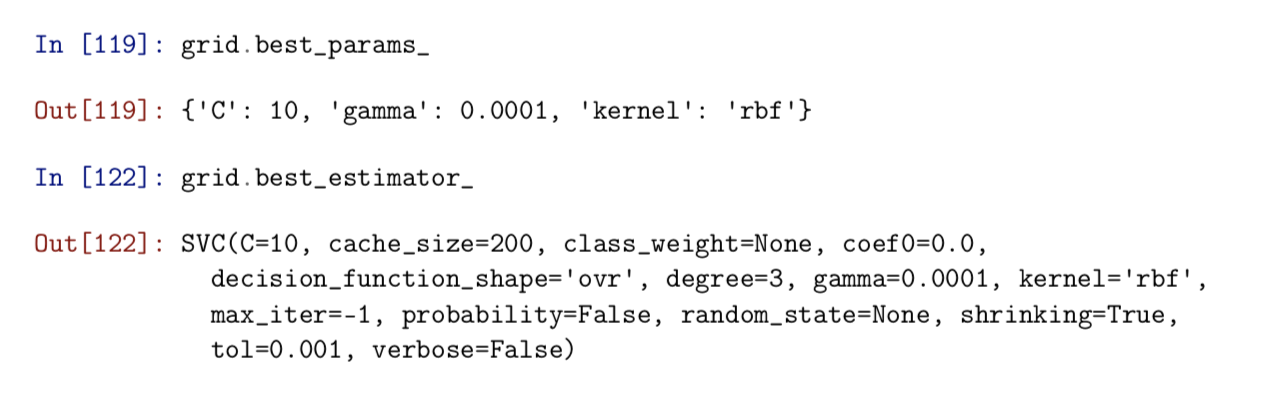
\includegraphics[width=50mm,scale=0.5]{imgs/params}}
\caption{best parameters \& estimator}
\label{fig}
\end{figure}

You can pull out the best parameters and estimators from grid search. With the adjusted parameters and normalization of the train test split data, we get a better accuracy for the model.

\begin{figure}[htbp]
\centerline{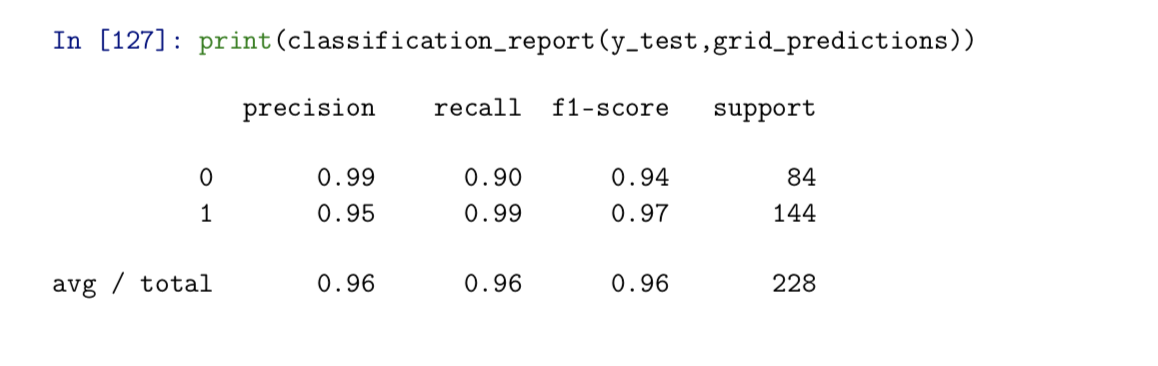
\includegraphics[width=50mm,scale=0.5]{imgs/class2}}
\caption{Prediction with  adjustment + normalization}
\label{fig}
\end{figure}

The SVC model does make sense in terms of mapping an example to a class with an accuracy of 96\%. With more time, I would extend this project to set up more classification models, including Neural Networks and K-Mean Clustering. With these different models, an obvious thing to do is compare and contrast the different models. An entire different report on the comparison would include errors margins, efficient margins and more data to describe the different techniques used. 

On the side, this project could extend to doing research and problem solving in other areas aside from the data sets we worked on. I would have loved to do a research project on how students past grades affect future classes, but that is for the future and a different time.



\end{document}
